\documentclass{beamer}
\usetheme{Hannover}
\setbeamersize{sidebar width left=0pt}
\usepackage[T1, T2A]{fontenc}
\usepackage[utf8]{inputenc}
\usepackage[russian]{babel}
\usepackage{hyperref}
\usepackage{graphicx}
\graphicspath{ {../Images/} }

\author{Григорий Матюхин}
\date{\today}
\title{Лабораторная работа \textnumero7.}
\subtitle{Управление журналами событий}

\begin{document}
\begin{frame}[plain]
	\titlepage
\end{frame}
\section{Цель работы}
\begin{frame}[plain]
	\frametitle{Цель работы}
	Получить навыки работы с журналами мониторинга различных событий в системе.
\end{frame}

\subsection{Мониторинг журнала системных событий в реальном времени}

\begin{frame}[plain]
	\frametitle{Мониторинг журнала системных событий в реальном времени}
	Запустите три вкладки терминала и в каждом из них получите полномочия администратора:
	На второй вкладке терминала запустите мониторинг системных событий в реальном времени:
	В третьей вкладке терминала вернитесь к учётной записи своего пользователя и попробуйте получить полномочия администратора, но введите неправильный пароль. Обратите внимание, что во второй вкладке терминала с мониторингом событий или ничего не отобразится, или появится сообщение \texttt{FAILED SU (to root) username ...}. Отображаемые на экране сообщения также фиксируются в файле \texttt{/var/log/messages}.
	\\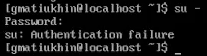
\includegraphics{1.png}
\end{frame}
\begin{frame}[plain]
	
\includegraphics{2.png}
\end{frame}
\begin{frame}[plain]
	В третьей вкладке терминала из оболочки пользователя введите \texttt{logger hello}. Во второй вкладке терминала с мониторингом событий вы увидите сообщение, которое также будет зафиксировано в файле /var/log/messages.
	\\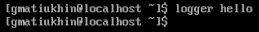
\includegraphics{3.png}
	\\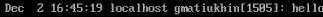
\includegraphics{4.png}
\end{frame}
\begin{frame}[plain]
	Во второй вкладке терминала с мониторингом остановите трассировку файла сообщений мониторинга реального времени. Затем запустите мониторинг сообщений безопасности (последние 20 строк соответствующего файла логов). Вы увидите сообщения, которые ранее были зафиксированы во время ошибки авторизации при вводе команды \texttt{su}.
	\\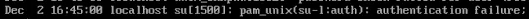
\includegraphics{5.png}
\end{frame}


\subsection{Изменение правил rsyslog.conf}
\begin{frame}[plain]
	\frametitle{Изменение правил rsyslog.conf}
	По умолчанию веб-служба не регистрирует свои сообщения через \texttt{rsyslog}, а пишет свой собственный журнал (в каталоге \texttt{/var/log/httpd}). Настройте регистрацию сообщений веб-службы через \texttt{syslog}, создав правило, регистрирующее отладочные сообщения в отдельном лог-файле. Для этого выполните следующие действия.
\end{frame}
\begin{frame}[plain]
	В первой вкладке терминала установите Apache, если он не был ранее инсталлирован:
	После окончания процесса установки запустите веб-службу:
	\\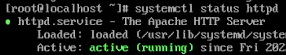
\includegraphics{6.png}
\end{frame}
\begin{frame}[plain]
	Во второй вкладке терминала посмотрите журнал сообщений об ошибках вебслужбы:
	\\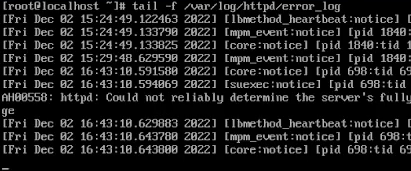
\includegraphics{7.png}
\end{frame}
\begin{frame}[plain]
	В третьей вкладке терминала получите полномочия администратора и в файле конфигурации \texttt{/etc/httpd/conf/httpd.conf} в конце добавьте следующую строку: \texttt{ErrorLog syslog:local1}. Здесь \texttt{local0} — \texttt{local7} — это «настраиваемые» средства (объекты), которые \texttt{syslog} предоставляет пользователю для регистрации событий приложения в системном журнале:
	\\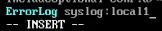
\includegraphics{8.png}
\end{frame}
\begin{frame}[plain]
	В каталоге \texttt{/etc/rsyslog.d} создайте файл мониторинга событий веб-службы. Открыв его на редактирование, пропишите в нём \texttt{local1.* -/var/log/httpd-error.log}. Эта строка позволит отправлять все сообщения, получаемые для объекта \texttt{local1} (который теперь используется службой \texttt{httpd}), в файл \texttt{/var/log/httpderror.log}:
	\\
\includegraphics{9.png}
\end{frame}
\begin{frame}[plain]
	Перейдите в первую вкладку терминала и перезагрузите конфигурацию \texttt{rsyslogd} и веб-службу. Все сообщения об ошибках веб-службы теперь будут записаны в файл \texttt{/var/log/httpd-error.log}, что можно наблюдать или в режиме реального времени, используя команду \texttt{tail} с соответствующими параметрами, или непосредственно просматривая указанный файл:
	\\
\includegraphics{10.png}
\end{frame}
\begin{frame}[plain]
	В третьей вкладке терминала создайте отдельный файл конфигурации для мониторинга отладочной информации. Открыв его на редактирование, пропишите в нём \texttt{*.debug /var/log/messages-debug}
	\\
\includegraphics{11.png}
\end{frame}
\begin{frame}[plain]
	В первой вкладке терминала снова перезапустите \texttt{rsyslogd}:
	Во второй вкладке терминала запустите мониторинг отладочной информации:
	В третьей вкладке терминала введите \texttt{logger -p daemon.debug "Daemon Debug Message"}:
	\\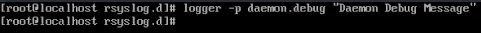
\includegraphics{12.png}
\end{frame}
\begin{frame}[plain]
	В терминале с мониторингом посмотрите сообщение отладки:
	\\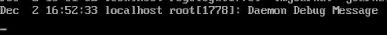
\includegraphics{13.png}
\end{frame}

\subsection{Использование journalctl}
\begin{frame}[plain]
	\frametitle{Использование journalctl}
	Во второй вкладке терминала посмотрите содержимое журнала с событиями с момента последнего запуска системы:
	\\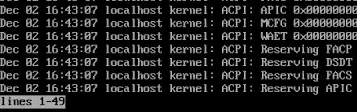
\includegraphics{14.png}
\end{frame}
\begin{frame}[plain]
	Просмотр содержимого журнала без использования пейджера:
	\\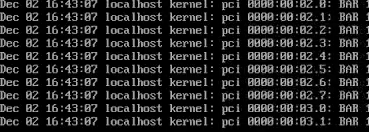
\includegraphics{15.png}
\end{frame}
\begin{frame}[plain]
	Режим просмотра журнала в реальном времени:
	\\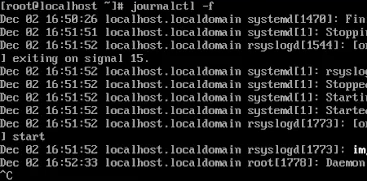
\includegraphics{16.png}
\end{frame}
\begin{frame}[plain]
	Просмотрите события для \texttt{UID0}:
	\\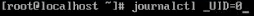
\includegraphics{17.png}
\end{frame}
\begin{frame}[plain]
	Для отображения последних 20 строк журнала введите:
	\\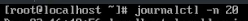
\includegraphics{18.png}
\end{frame}
\begin{frame}[plain]
	Для просмотра только сообщений об ошибках введите:
	\\
\includegraphics{19.png}
\end{frame}
\begin{frame}[plain]
	Если вы хотите просмотреть сообщения журнала, записанные за определённый период времени, вы можете использовать параметры \texttt{--since} и \texttt{--until}. Обе опции принимают параметр времени в формате \texttt{YYYY-MM-DD hh:mm:ss}. Кроме того, вы можете использовать \texttt{yesterday}, \texttt{today} и \texttt{tomorrow} в качестве параметров. Например, для просмотра всех сообщений со вчерашнего дня введите:
	\\
\includegraphics{20.png}
\end{frame}
\begin{frame}[plain]
	Если вы хотите показать все сообщения с ошибкой приоритета, которые были зафиксированы со вчерашнего дня, то используйте:
	\\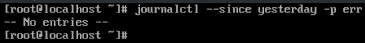
\includegraphics{21.png}
\end{frame}
\begin{frame}[plain]
	Если вам нужна детальная информация, то используйте \texttt{journalctl -o verbose}:
	\\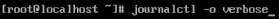
\includegraphics{22.png}
\end{frame}
\begin{frame}[plain]
	Для просмотра дополнительной информации о модуле sshd введите \texttt{journalctl \_SYSTEMD\_UNIT=sshd.service}:
	\\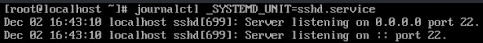
\includegraphics{23.png}
\end{frame}

\subsection{Постоянный журнал journald}
\begin{frame}[plain]
	\frametitle{Постоянный журнал journald}
	По умолчанию журнал journald хранит сообщения в оперативной памяти системы и записи доступны в каталоге \texttt{/run/log/journal} только до перезагрузки системы. Для того чтобы сделать журнал \texttt{journald} постоянным, выполните следующие действия:
\end{frame}
\begin{frame}[plain]
	Запустите терминал и получите полномочия администратора:
	Создайте каталог для хранения записей журнала:
	\label{access} Скорректируйте права доступа для каталога \texttt{/var/log/journal}, чтобы \texttt{journald} смог записывать в него информацию:
	\\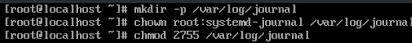
\includegraphics{24.png}
\end{frame}
\begin{frame}[plain]
	Для принятия изменений необходимо или перезагрузить систему (перезапустить службу \texttt{systemd-journald} недостаточно), или использовать команду \texttt{killall -USR1 systemd-journald}:
	\\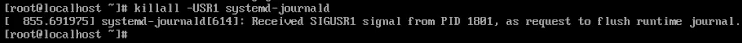
\includegraphics{25.png}
\end{frame}

\section{Вывод}
\begin{frame}[plain]
	\frametitle{Вывод}
	В ходе выполнения данной работы я получил навыки работы с журналами мониторинга различных событий в системе.
\end{frame}

\end{document}
